\bta{天体和行星的运行}

\begin{enumerate}[leftmargin=0em]
\renewcommand{\labelenumi}{\arabic{enumi}.}
% A(\Alph) a(\alph) I(\Roman) i(\roman) 1(\arabic)
%设定全局标号series=example	%引用全局变量resume=example
%[topsep=-0.3em,parsep=-0.3em,itemsep=-0.3em,partopsep=-0.3em]
%可使用leftmargin调整列表环境左边的空白长度 [leftmargin=0em]
\item
\exwhere{$ 2019 $年物理天津卷}
$ 2018 $年$ 12 $月$ 8 $日,肩负着亿万中华儿女探月飞天梦想的嫦娥四号探测器成功发射,“实现人类航天器首次在月球背面巡视探测,率先在月背刻上了中国足迹”。已知月球的质量为、半径为,探测器的质量为,引力常量为,嫦娥四号探测器围绕月球做半径为的匀速圆周运动时,探测器的 \xzanswer{C} 


\fourchoices
{周期为$\sqrt { \frac { 4 \pi ^ { 2 } r ^ { 3 } } { G M } }$}
{动能为$\frac { G M m } { 2 R }$}
{角速度为$\sqrt { \frac { G m } { r ^ { 3 } } }$}
{向心加速度为$\frac { G M } { R ^ { 2 } }$}




\item 
\exwhere{$ 2013 $年福建卷}
设太阳质量为$ M $,某行星绕太阳公转周期为$ T $,轨道可视作半径为$ r $的圆。已知万有引力常量为$ G $,则描述该行星运动的上述物理量满足 \xzanswer{A} 

\fourchoices
{$ G M = \frac { 4 \pi ^ { 2 } r ^ { 3 } } { T ^ { 2 } } $}
{$ G M = \frac { 4 \pi ^ { 2 } r ^ { 2 } } { T ^ { 2 } } $}
{$ G M = \frac { 4 \pi ^ { 2 } r ^ { 2 } } { T ^ { 3 } } $}
{$ G M = \frac { 4 \pi r ^ { 3 } } { T ^ { 2 } } $}


\item
\exwhere{$ 2013 $年上海卷}
小行星绕恒星运动,恒星均匀地向四周辐射能量,质量缓慢减小,可认为小行星在绕恒星运动一周的过程中近似做圆周运动。则经过足够长的时间后,小行星运动的 \xzanswer{A} 

\fourchoices
{半径变大	 }
{速率变大}
{角速度变大 }
{加速度变大}



\item
\exwhere{$ 2014 $年理综浙江卷}
长期以来“卡戎星($ Charon $)”被认为是冥王星唯一的卫星,它的公转轨道半径$ r_1=19600 \ km $,公转周期$ T_{1} =6.39 $天。$ 2006 $年$ 3 $月,天文学家新发现两颗冥王星的小卫星,其中一颗的公转轨道半径$ r_2=48000 \ km $,则它的公转周期$ T_{2} $最接近于 \xzanswer{B} 

\fourchoices
{$ 15 $天}
{$ 25 $天}
{$ 35 $天}
{$ 45 $天}



\item 
\exwhere{$ 2013 $年江苏卷}
火星和木星沿各自的椭圆轨道绕太阳运行,根据开普勒行星运动定律可知 \xzanswer{C} 



\fourchoices
{太阳位于木星运行轨道的中心}
{火星和木星绕太阳运行速度的大小始终相等}
{火星与木星公转周期之比的平方等于它们轨道半长轴之比的立方}
{相同时间内,火星与太阳连线扫过的面积等于木星与太阳连线扫过的面积}

\item 
\exwhere{$ 2014 $年物理江苏卷}
已知地球的质量约为火星质量的 $ 10 $ 倍,地球的半径约为火星半径的 $ 2 $ 倍,则航天器在火星表面附近绕火星做匀速圆周运动的速率约为 \xzanswer{A} 

\fourchoices
{$ 3 . 5 $ $ km / s $}
{$ 5 . 0 $ $ km / s $}
{$ 17 . 7 $ $ km / s $}
{$ 35 . 2 $ $ km / s $}

\newpage
\item 
\exwhere{$ 2012 $年物理江苏卷}
$ 2011 $年$ 8 $月,“嫦娥二号”成功进入了环绕“日地拉格朗日点”的轨道,我国成为世界上第三个造访该点的国家。 如图所示,该拉格朗日点位于太阳和地球连线的延长线上,一飞行器处于该点,在几乎不消耗燃料的情况下与地球同步绕太阳做圆周运动,则此飞行器的 \xzanswer{AB} 
\begin{figure}[h!]
\centering
\includesvg[width=0.17\linewidth]{picture/svg/598}
\end{figure}


\fourchoices
{线速度大于地球的线速度}
{向心加速度大于地球的向心加速度}
{向心力仅由太阳的引力提供}
{向心力仅由地球的引力提供}





\item 
\exwhere{$ 2012 $年理综浙江卷}
如图所示,在火星与木星轨道之间有一小行星带。假设该带中的小行星只受到太阳的引力,并绕太阳做匀速圆周运动。下列说法正确的是 \xzanswer{C} 
\begin{figure}[h!]
\centering
\includesvg[width=0.4\linewidth]{picture/svg/599}
\end{figure}

\fourchoices
{太阳对各小行星的引力相同}
{各小行星绕太阳运动的周期均小于一年}
{小行星带内侧小行星的向心加速度值大于外侧小行星的向心加速度值}
{小行星带内各小行星圆周运动的线速度值大于地球公转的线速度值}







\item 
\exwhere{$ 2011 $年物理江苏卷}
一行星绕恒星作圆周运动。由天文观测可得,其运动周期为$ T $,速度为$ v $,引力常量为$ G $,则 \xzanswer{ACD} 

\fourchoices
{恒星的质量为 $\frac { v ^ { 3 } T } { 2 \pi G }$ }
{行星的质量为$\frac { 4 \pi ^ { 2 } v ^ { 3 } } { G T ^ { 2 } }$}
{行星运动的轨道半径为 $\frac { v T } { 2 \pi }$ }
{行星运动的加速度为$\frac { 2 \pi v } { T }$}




\item 
\exwhere{$ 2012 $年理综广东卷}
如图所示,飞船从轨道$ 1 $变轨至轨道$ 2 $。若飞船在两轨道上都做匀速圆周运动,不考虑质量变化,相对于在轨道$ 1 $上,飞船在轨道$ 2 $上的 \xzanswer{CD} 
\begin{figure}[h!]
\centering
\includesvg[width=0.23\linewidth]{picture/svg/600}
\end{figure}

\fourchoices
{动能大}
{向心加速度大}
{运行周期长}
{角速度小}



\item 
\exwhere{$ 2017 $年新课标$ \lmd{2} $卷}
如图,海王星绕太阳沿椭圆轨道运动,$ P $为近日点,$ Q $为远日点,$ M $,$ N $为轨道短轴的两个端点,运行的周期为$ T_{0} $,若只考虑海王星和太阳之间的相互作用,则海王星在从$ P $经过$ M $,$ Q $到$ N $的运动过程中 \xzanswer{CD} 
\begin{figure}[h!]
\centering
\includesvg[width=0.23\linewidth]{picture/svg/601}
\end{figure}

\fourchoices
{从$ P $到$ M $所用的时间等于}
{从$ Q $到$ N $阶段,机械能逐渐变大}
{从$ P $到$ Q $阶段,速率逐渐变小}
{从$ M $到$ N $阶段,万有引力对它先做负功后做正功}



\item 
\exwhere{$ 2018 $年海南卷}
土星与太阳的距离是火星与太阳距离的$ 6 $倍多。由此信息可知 \xzanswer{B} 

\fourchoices
{土星的质量比火星的小}
{土星运行的速率比火星的小}
{土星运行的周期比火星的小}
{土星运行的角速度大小比火星的大}


\item
\exwhere{$ 2017 $年浙江选考卷}
如图所示,设行星绕太阳的运动是匀速圆周运动,金星自身的半径是火星的$ n $倍,质量为火星的$ k $倍,不考虑行星自转的影响,则 \xzanswer{B} 
\begin{figure}
\centering
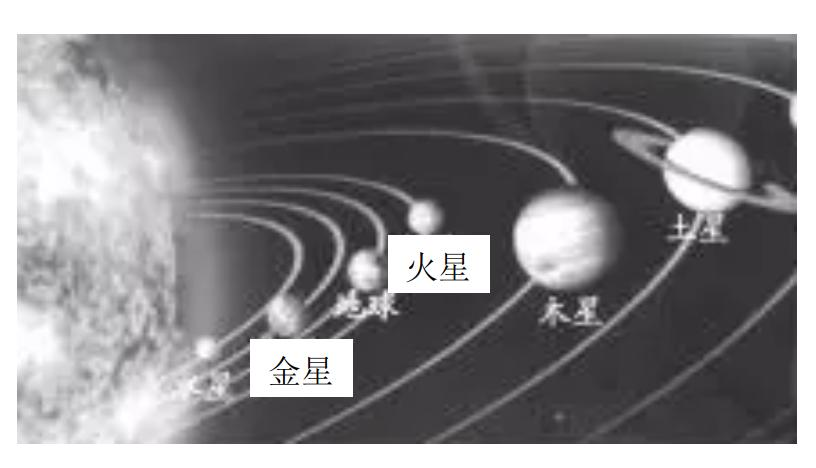
\includegraphics[width=0.3\linewidth]{picture/screenshot005}
\end{figure}

\fourchoices
{金星表面的重力加速度是火星的 $\frac { k } { n }$}
{金星的第一宇宙速度是火星的$\sqrt { \frac { k } { n } }$}
{金星绕太阳运动的加速度比火星小}
{金星绕太阳运动的周期比火星大}



\item 
\exwhere{$ 2013 $年山东卷}
双星系统由两颗恒星组成,两恒星在相互引力的作用下,分别围绕其连线上的某一点做周期相同的匀速圆周运动。研究发现,双星系统演化过程中,两星的总质量、距离和周期均可能发生变化。若某双星系统中两星做圆周运动的周期为$ T $,经过一段时间演化后,两星总质量变为原来的$ k $倍,双星之间的距离变为原来的$ n $倍,则此时圆周运动的周期为 \xzanswer{B} 



\fourchoices
{$ \sqrt { \frac { n ^ { 3 } } { k ^ { 2 } } } T $}
{$ \sqrt { \frac { n ^ { 3 } } { k } } T $}
{$ \sqrt { \frac { n ^ { 2 } } { k } } T $}
{$ \sqrt { \frac { n } { k } } T $}




\item
\exwhere{$ 2013 $年四川卷}
迄今发现的二百余颗太阳系外行星大多不适宜人类居住,绕恒星“$ Gliese581 $”运行的行星“$ Gl-581c $”却很值得我们期待。该行星的温度在$ 0 \ \celsius $到$ 40 \ \celsius $之间、质量是地球的$ 6 $倍、直径是地球的$ 1.5 $倍、公转周期为$ 13 $个地球日。“$ Gliese581 $”的质量是太阳质量的$ 0.31 $倍。设该行星与地球均视为质量分布均匀的球体,绕其中心天体做匀速圆周运动,则 \xzanswer{B} 

\fourchoices
{在该行星和地球上发射卫星的第一宇宙速度相同}
{如果人到了该行星,其体重是地球上的$ 2 \frac{ 2 }{ 3 } $倍}
{该行星与“$ Gliese581 $”的距离是日地距离的$\sqrt { \frac { 13 } { 365 } }$倍}
{由于该行星公转速率比地球大,地球上的米尺如果被带上该行星,其长度一定会变短}






\item 
\exwhere{$ 2011 $年理综四川卷}
据报道,天文学家近日发现了一颗距地球$ 40 $光年的“超级地球”,名为“$ 55Cancri $ $ e $”,该行星绕母星(中心天体)运行的周期约为地球绕太阳运行周期的$ 1/480 $,母星的体积约为太阳的$ 60 $倍。假设母星与太阳密度相同,“$ 55 $ $ Cancri $ $ e $”与地球均做匀速圆周运动,则“$ 55 $ $ Cancri $ $ e $”与地球的 \xzanswer{B} 

\fourchoices
{轨道半径之比约为 $\sqrt [ 3 ] { \frac { 60 } { 480 } }$ 	 }
{轨道半径之比约为$\sqrt [ 3 ] { \frac { 60 } { 480 ^ { 2 } } }$}
{向心加速度之比约为$\sqrt [ 3 ] { 60 \times 480 ^ { 2 } }$ }
{向心加速度之比约为$\sqrt [ 3 ] { 60 \times 480 }$}



\item
\exwhere{$ 2011 $年理综浙江卷}
为了探测$ X $星球,载着登陆舱的探测飞船在以该星球中心为圆心,半径为$ r_{1} $的圆轨道上运动,周期为$ T_{1} $。总质量为$ m_{1} $。随后登陆舱脱离飞船,变轨到离星球更近的半径为$ r_{2} $的圆轨道上运动,此时登陆舱的质量为$ m_{2} $则 \xzanswer{AD} 

\fourchoices
{$ X $星球的质量为$M = \frac { 4 \pi ^ { 2 } r _ { 1 } ^ { 3 } } { G T _ { 1 } ^ { 2 } }$}
{$ X $星球表面的重力加速度为$g _ { x } = \frac { 4 \pi ^ { 2 } r _ { 1 } } { T _ { 1 } ^ { 2 } }$}
{登陆舱在$ r_{1} $与$ r_{2} $轨道上运动时的速度大小之比为$\frac { v _ { 1 } } { v _ { 2 } } = \sqrt { \frac { m _ { 1 } r _ { 2 } } { m _ { 2 } r _ { 1 } } }$}
{登陆舱在半径为$ r_{2} $轨道上做圆周运动的周期为$T _ { 2 } = T _ { 1 } \sqrt { \frac { r _ { 2 } ^ { 3 } } { r _ { 1 } ^ { 3 } } }$}



\item 
\exwhere{$ 2011 $年理综重庆卷}
某行星和地球绕太阳公转的轨道均可视为圆。每过$ N $年,该行星会运行到日地连线的延长线上,如图所示。该行星与地球的公转半径比为 \xzanswer{B} 
\begin{figure}[h!]
\centering
\includesvg[width=0.23\linewidth]{picture/svg/602}
\end{figure}

\fourchoices
{$ \left( \frac { N + 1 } { N } \right) ^ { \frac { 2 } { 3 } } $}
{$ \left( \frac { N } { N - 1 } \right) ^ { \frac { 2 } { 3 } } $}
{$ \left( \frac { N + 1 } { N } \right) ^ { \frac { 3 } { 2 } } $}
{$ \left( \frac { N } { N - 1 } \right) ^ { \frac { 3 } { 2 } } $}

\item 
\exwhere{$ 2014 $年理综新课标\lmd{1}卷}
太阳系各行星几乎在同一平面内沿同一方向绕太阳做圆周运动,当地球恰好运行到某个行星和太阳之间,且三者几乎成一条直线的现象,天文学成为“行星冲日”。据报道,$ 2014 $年各行星冲日时间分别是:$ 1 $月$ 6 $日木星冲日,$ 4 $月$ 9 $日火星冲日,$ 5 $月$ 11 $日土星冲日,$ 8 $月$ 29 $日海王星冲日,$ 10 $月$ 8 $日天王星冲日,已知地球轨道以外行星绕太阳运动的轨道半径如下表所示,则下列判断正确的是 \xzanswer{BD} 
\begin{table}[h!]
\centering 
\begin{tabular}{|c|c|c|c|c|c|c|}
\hline 
& 地球 & 火星 & 木星 & 土星 & 天王星 & 海王星
 \\
\hline
轨道半径(AU) & 1.0 & 1.5 & 5.2 & 9.5 & 19 & 30\\ 
\hline 
\end{tabular}
\end{table} 

\fourchoices
{各地外行星每年都会出现冲日现象}
{在$ 2015 $年内一定会出现木星冲日}
{天王星相邻两次的冲日的时间是土星的一半}
{地外行星中,海王星相邻两次冲日间隔时间最短}




\item 
\exwhere{$ 2015 $年理综新课标 \lmd{1} 卷}
我国发射的“嫦娥三号”登月探测器靠近月球后,先在月球表面附近的近似圆轨道上绕月运行;然后经过一系列过程,在离月面$ 4 \ m $高处做一次悬停(可认为是相对于月球静止);最后关闭发动机,探测器自由下落。已知探测器的质量约为$ 1.3 \times 10^3 \ kg $,地球质量约为月球的$ 81 $倍,地球半径约为月球的$ 3.7 $倍,地球表面的重力加速度大小约为$ 9.8 \ m/s^{2} $,则此探测器 \xzanswer{BD} 

\fourchoices
{在着陆前的瞬间,速度大小约为$ 8.9 \ m/s $}
{悬停时受到的反冲作用力约为$ 2 \times 10^3 \ N $}
{从离开近月圆轨道到着陆这段时间内,机械能守恒}
{在近月圆轨道上运行的线速度小于人造卫星在近地圆轨道上运行的线速度}


\item
\exwhere{$ 2015 $年理综天津卷}
$ P_{1} $、$ P_{2} $为相距遥远的两颗行星,距各自表面相同高度处各有一颗卫星$ s_{1} $、$ s_{2} $做匀速圆周运动,图中纵坐标表示行星对周围空间各处物体的引力产生的加速度$ a $,横坐标表示物体到行星中心的距离$ r $的平方,两条曲线分别表示$ P_{1} $、$ P_{2} $周围的$ a $与$ r^{2} $的反比关系,它们左端点横坐标相同,则 \xzanswer{AC} 
\begin{figure}[h!]
\centering
\includesvg[width=0.23\linewidth]{picture/svg/603}
\end{figure}


\fourchoices
{$ P_{1} $的平均密度比$ P_{2} $的大}
{$ P_{1} $的第一宇宙速度比$ P_{2} $的小}
{$ s_{1} $的向心加速度比$ s_{2} $的大}
{$ s_{1} $的公转周期比$ s_{2} $的大}



\item 
\exwhere{$ 2011 $年理综安徽卷}
\begin{enumerate}
\renewcommand{\labelenumi}{\arabic{enumi}.}
% A(\Alph) a(\alph) I(\Roman) i(\roman) 1(\arabic)
%设定全局标号series=example	%引用全局变量resume=example
%[topsep=-0.3em,parsep=-0.3em,itemsep=-0.3em,partopsep=-0.3em]
%可使用leftmargin调整列表环境左边的空白长度 [leftmargin=0em]
\item
开普勒行星运动第三定律指出:行星绕太阳运动的椭圆轨道的半长轴$ a $的三次方与它的公转周期$ T $的二次方成正比,即$\frac { a ^ { 3 } } { T ^ { 2 } } = k$,$ k $是一个对所有行星都相同的常量。将行星绕太阳的运动按圆周运动处理,请你推导出太阳系中该常量$ k $的表达式。已知引力常量为$ G $,太阳的质量为$ M_{ \text{太} } $。
\item 
开普勒定律不仅适用于太阳系,它对一切具有中心天体的引力系统(如地月系统)都成立。经测定月地距离为$ 3.84 \times 10^8\ m $,月球绕地球运动的周期为$ 2.36 \times 10^6\ s $,试计算地球的质量$ M_{ \text{地} } $。($ G=6.67 \times 10^{-11} \ N \cdot m^{2} /kg^{2} $,结果保留一位有效数字)



\end{enumerate}

\banswer{
\begin{enumerate}
\renewcommand{\labelenumi}{\arabic{enumi}.}
% A(\Alph) a(\alph) I(\Roman) i(\roman) 1(\arabic)
%设定全局标号series=example	%引用全局变量resume=example
%[topsep=-0.3em,parsep=-0.3em,itemsep=-0.3em,partopsep=-0.3em]
%可使用leftmargin调整列表环境左边的空白长度 [leftmargin=0em]
\item
$k = \frac { G } { 4 \pi ^ { 2 } } M _ { \text{太} }$
\item 
$M _ { \text{地} } = 6 \times 10 ^ { 24 } \ \mathrm { kg }$ \qquad ($M _ { \text{地} } = 5 \times 10 ^ { 24 } \ \mathrm { kg }$ 也算对)

\end{enumerate}


}







\end{enumerate}

